 \documentclass[handout]{beamer}
%\documentclass[handout]{beamer}
\usepackage{graphicx, color}
\usepackage{tikz}
\usepackage{subfigure}

% Use something like:
% % Use something like:
% % Use something like:
% \input{../../macros}

% groupings of objects.
\newcommand{\set}[1]{\ensuremath{\left\{ #1 \right\}}}
\newcommand{\seq}[1]{\ensuremath{\left(#1\right)}}
\newcommand{\ang}[1]{\ensuremath{\langle#1\rangle}}
\newcommand{\tuple}[1]{\ensuremath{\left(#1\right)}}
\newcommand{\size}[1]{\ensuremath{\left| #1\right|}}

% numerical shortcuts.
\newcommand{\abs}[1]{\ensuremath{\left| #1\right|}}
\newcommand{\floor}[1]{\ensuremath{\left\lfloor #1 \right\rfloor}}
\newcommand{\ceil}[1]{\ensuremath{\left\lceil #1 \right\rceil}}

% linear algebra shortcuts.
\newcommand{\change}{\ensuremath{\Delta}}
\newcommand{\norm}[1]{\ensuremath{\left\| #1\right\|}}
\newcommand{\dprod}[1]{\ensuremath{\langle#1\rangle}}
\newcommand{\linspan}[1]{\ensuremath{\langle#1\rangle}}
\newcommand{\conj}[1]{\ensuremath{\overline{#1}}}
\newcommand{\der}{\ensuremath{\frac{d}{dx}}}
\newcommand{\lap}{\ensuremath{\Delta}}
\newcommand{\kron}{\ensuremath{\otimes}}
\newcommand{\nperp}{\ensuremath{\nvdash}}

\newcommand{\mat}[1]{\left[ \begin{smallmatrix}#1 \end{smallmatrix} \right]}

% derivatives and limits
\newcommand{\partder}[2]{\ensuremath{\frac{\partial #1}{\partial #2}}}
\newcommand{\partdern}[3]{\ensuremath{\frac{\partial^{#3} #1}{\partial #2^{#3}}}}
\newcommand{\gradient}{\ensuremath{\nabla}}
\newcommand{\subdifferential}{\ensuremath{\partial}}

% Arrows
\newcommand{\diverge}{\ensuremath{\nearrow}}
\newcommand{\notto}{\ensuremath{\nrightarrow}}
\newcommand{\up}{\ensuremath{\uparrow}}
\newcommand{\down}{\ensuremath{\downarrow}}
% gets and gives are defined!

% ordering operators
\newcommand{\oleq}{\preceq}
\newcommand{\ogeq}{\succeq}

% programming and logic operators
\newcommand{\dfn}{:=}
\newcommand{\assign}{:=}
\newcommand{\co}{\ co\ }
\newcommand{\en}{\ en\ }


% logic operators
\newcommand{\xor}{\ensuremath{\oplus}}
\newcommand{\Land}{\ensuremath{\bigwedge}}
\newcommand{\Lor}{\ensuremath{\bigvee}}
\newcommand{\finish}{\ensuremath{\Box}}
\newcommand{\contra}{\ensuremath{\Rightarrow \Leftarrow}}
\newcommand{\iseq}{\ensuremath{\stackrel{_?}{=}}}


% Set theory
\newcommand{\symdiff}{\ensuremath{\Delta}}
\newcommand{\union}{\ensuremath{\cup}}
\newcommand{\inters}{\ensuremath{\cap}}
\newcommand{\Union}{\ensuremath{\bigcup}}
\newcommand{\Inters}{\ensuremath{\bigcap}}
\newcommand{\nullSet}{\ensuremath{\phi}}


% graph theory
\newcommand{\nbd}{\Gamma}

% Script alphabets
% For reals, use \Re

% greek letters
\newcommand{\eps}{\ensuremath{\epsilon}}
\newcommand{\del}{\ensuremath{\delta}}
\newcommand{\ga}{\ensuremath{\alpha}}
\newcommand{\gb}{\ensuremath{\beta}}
\newcommand{\gd}{\ensuremath{\del}}
\newcommand{\gp}{\ensuremath{\pi}}
\newcommand{\gf}{\ensuremath{\phi}}
\newcommand{\gh}{\ensuremath{\eta}}
\newcommand{\gF}{\ensuremath{\Phi}}
\newcommand{\gl}{\ensuremath{\lambda}}
\newcommand{\gm}{\ensuremath{\mu}}
\newcommand{\gn}{\ensuremath{\nu}}
\newcommand{\gr}{\ensuremath{\rho}}
\newcommand{\gs}{\ensuremath{\sigma}}
\newcommand{\gt}{\ensuremath{\theta}}
\newcommand{\gx}{\ensuremath{\xi}}

\newcommand{\sw}{\ensuremath{\sigma}}
\newcommand{\SW}{\ensuremath{\Sigma}}
\newcommand{\ew}{\ensuremath{\lambda}}
\newcommand{\EW}{\ensuremath{\Lambda}}

\newcommand{\Del}{\ensuremath{\Delta}}
\newcommand{\gD}{\ensuremath{\Delta}}
\newcommand{\gG}{\ensuremath{\Gamma}}
\newcommand{\gO}{\ensuremath{\Omega}}
\newcommand{\gS}{\ensuremath{\Sigma}}

% Bold english letters.
\newcommand{\bA}{\ensuremath{\mathbf{A}}}
\newcommand{\bB}{\ensuremath{\mathbf{B}}}
\newcommand{\bC}{\ensuremath{\mathbf{C}}}
\newcommand{\bD}{\ensuremath{\mathbf{D}}}
\newcommand{\bE}{\ensuremath{\mathbf{E}}}
\newcommand{\bF}{\ensuremath{\mathbf{F}}}
\newcommand{\bG}{\ensuremath{\mathbf{G}}}
\newcommand{\bH}{\ensuremath{\mathbf{H}}}
\newcommand{\bI}{\ensuremath{\mathbf{I}}}
\newcommand{\bJ}{\ensuremath{\mathbf{J}}}
\newcommand{\bK}{\ensuremath{\mathbf{K}}}
\newcommand{\bL}{\ensuremath{\mathbf{L}}}
\newcommand{\bM}{\ensuremath{\mathbf{M}}}
\newcommand{\bN}{\ensuremath{\mathbf{N}}}
\newcommand{\bO}{\ensuremath{\mathbf{O}}}
\newcommand{\bP}{\ensuremath{\mathbf{P}}}
\newcommand{\bQ}{\ensuremath{\mathbf{Q}}}
\newcommand{\bR}{\ensuremath{\mathbf{R}}} % PROSPER defines \R
\newcommand{\bS}{\ensuremath{\mathbf{S}}}
\newcommand{\bT}{\ensuremath{\mathbf{T}}}
\newcommand{\bU}{\ensuremath{\mathbf{U}}}
\newcommand{\bV}{\ensuremath{\mathbf{V}}}
\newcommand{\bW}{\ensuremath{\mathbf{W}}}
\newcommand{\bX}{\ensuremath{\mathbf{X}}}
\newcommand{\bY}{\ensuremath{\mathbf{Y}}}
\newcommand{\bZ}{\ensuremath{\mathbf{Z}}}
\newcommand{\bba}{\ensuremath{\mathbf{a}}}
\newcommand{\bbb}{\ensuremath{\mathbf{b}}}
\newcommand{\bbc}{\ensuremath{\mathbf{c}}}
\newcommand{\bbd}{\ensuremath{\mathbf{d}}}
\newcommand{\bbe}{\ensuremath{\mathbf{e}}}
\newcommand{\bbf}{\ensuremath{\mathbf{f}}}
\newcommand{\bbg}{\ensuremath{\mathbf{g}}}
\newcommand{\bbh}{\ensuremath{\mathbf{h}}}
\newcommand{\bbk}{\ensuremath{\mathbf{k}}}
\newcommand{\bbl}{\ensuremath{\mathbf{l}}}
\newcommand{\bbm}{\ensuremath{\mathbf{m}}}
\newcommand{\bbn}{\ensuremath{\mathbf{n}}}
\newcommand{\bbp}{\ensuremath{\mathbf{p}}}
\newcommand{\bbq}{\ensuremath{\mathbf{q}}}
\newcommand{\bbr}{\ensuremath{\mathbf{r}}}
\newcommand{\bbs}{\ensuremath{\mathbf{s}}}  % TIPA defines \s and LaTeX \ss!
\newcommand{\bbt}{\ensuremath{\mathbf{t}}}
\newcommand{\bbu}{\ensuremath{\mathbf{u}}}
\newcommand{\bbv}{\ensuremath{\mathbf{v}}}
\newcommand{\bbw}{\ensuremath{\mathbf{w}}}
\newcommand{\bbx}{\ensuremath{\mathbf{x}}}
\newcommand{\bby}{\ensuremath{\mathbf{y}}}
\newcommand{\bbz}{\ensuremath{\mathbf{z}}}
\newcommand{\0}{\ensuremath{\mathbf{0}}}
\newcommand{\1}{\ensuremath{\mathbf{1}}}


% Formatting shortcuts
\newcommand{\red}[1]{\textcolor{red}{#1}}
\newcommand{\green}[1]{\textcolor{green}{#1}}
\newcommand{\magenta}[1]{\textcolor{magenta}{#1}}
\newcommand{\orange}[1]{\textcolor{orange}{#1}}
\newcommand{\gray}[1]{\textcolor{gray}{#1}}
\newcommand{\blue}[1]{\textcolor{blue}{#1}}
\newcommand{\htext}[2]{\texorpdfstring{#1}{#2}}

% Statistics
\newcommand{\distr}{\ensuremath{\sim}}
\newcommand{\stddev}{\ensuremath{\sigma}}
\newcommand{\covmatrix}{\ensuremath{\Sigma}}
\newcommand{\mean}{\ensuremath{\mu}}
\newcommand{\param}{\ensuremath{\gt}}
\newcommand{\ftr}{\ensuremath{\phi}}

% General utility
\newcommand{\todo}[1]{\textbf{[TODO]}] \footnote{TODO: #1}}
\newcommand{\exclaim}[1]{{\textbf{\textit{#1}}}}
\newcommand{\tbc}{[\textbf{Incomplete}]}
\newcommand{\chk}{[\textbf{Check}]}
\newcommand{\oprob}{[\textbf{OP}]:}
\newcommand{\core}[1]{\textbf{Core Idea:}}
\newcommand{\why}{[\textbf{Find proof}]}
\newcommand{\opt}[1]{\textit{#1}}


\renewcommand{\~}{\htext{$\sim$}{~}}

\DeclareMathOperator*{\argmin}{arg\,min}
\DeclareMathOperator*{\argmax}{arg\,max}

% Items pertaining to the headed list.
\newcommand{\headeditem}[1]{\item\textbf{#1}}
\newcommand{\headedsubitem}[1]{\subitem\textbf{#1}}



% groupings of objects.
\newcommand{\set}[1]{\ensuremath{\left\{ #1 \right\}}}
\newcommand{\seq}[1]{\ensuremath{\left(#1\right)}}
\newcommand{\ang}[1]{\ensuremath{\langle#1\rangle}}
\newcommand{\tuple}[1]{\ensuremath{\left(#1\right)}}
\newcommand{\size}[1]{\ensuremath{\left| #1\right|}}

% numerical shortcuts.
\newcommand{\abs}[1]{\ensuremath{\left| #1\right|}}
\newcommand{\floor}[1]{\ensuremath{\left\lfloor #1 \right\rfloor}}
\newcommand{\ceil}[1]{\ensuremath{\left\lceil #1 \right\rceil}}

% linear algebra shortcuts.
\newcommand{\change}{\ensuremath{\Delta}}
\newcommand{\norm}[1]{\ensuremath{\left\| #1\right\|}}
\newcommand{\dprod}[1]{\ensuremath{\langle#1\rangle}}
\newcommand{\linspan}[1]{\ensuremath{\langle#1\rangle}}
\newcommand{\conj}[1]{\ensuremath{\overline{#1}}}
\newcommand{\der}{\ensuremath{\frac{d}{dx}}}
\newcommand{\lap}{\ensuremath{\Delta}}
\newcommand{\kron}{\ensuremath{\otimes}}
\newcommand{\nperp}{\ensuremath{\nvdash}}

\newcommand{\mat}[1]{\left[ \begin{smallmatrix}#1 \end{smallmatrix} \right]}

% derivatives and limits
\newcommand{\partder}[2]{\ensuremath{\frac{\partial #1}{\partial #2}}}
\newcommand{\partdern}[3]{\ensuremath{\frac{\partial^{#3} #1}{\partial #2^{#3}}}}
\newcommand{\gradient}{\ensuremath{\nabla}}
\newcommand{\subdifferential}{\ensuremath{\partial}}

% Arrows
\newcommand{\diverge}{\ensuremath{\nearrow}}
\newcommand{\notto}{\ensuremath{\nrightarrow}}
\newcommand{\up}{\ensuremath{\uparrow}}
\newcommand{\down}{\ensuremath{\downarrow}}
% gets and gives are defined!

% ordering operators
\newcommand{\oleq}{\preceq}
\newcommand{\ogeq}{\succeq}

% programming and logic operators
\newcommand{\dfn}{:=}
\newcommand{\assign}{:=}
\newcommand{\co}{\ co\ }
\newcommand{\en}{\ en\ }


% logic operators
\newcommand{\xor}{\ensuremath{\oplus}}
\newcommand{\Land}{\ensuremath{\bigwedge}}
\newcommand{\Lor}{\ensuremath{\bigvee}}
\newcommand{\finish}{\ensuremath{\Box}}
\newcommand{\contra}{\ensuremath{\Rightarrow \Leftarrow}}
\newcommand{\iseq}{\ensuremath{\stackrel{_?}{=}}}


% Set theory
\newcommand{\symdiff}{\ensuremath{\Delta}}
\newcommand{\union}{\ensuremath{\cup}}
\newcommand{\inters}{\ensuremath{\cap}}
\newcommand{\Union}{\ensuremath{\bigcup}}
\newcommand{\Inters}{\ensuremath{\bigcap}}
\newcommand{\nullSet}{\ensuremath{\phi}}


% graph theory
\newcommand{\nbd}{\Gamma}

% Script alphabets
% For reals, use \Re

% greek letters
\newcommand{\eps}{\ensuremath{\epsilon}}
\newcommand{\del}{\ensuremath{\delta}}
\newcommand{\ga}{\ensuremath{\alpha}}
\newcommand{\gb}{\ensuremath{\beta}}
\newcommand{\gd}{\ensuremath{\del}}
\newcommand{\gp}{\ensuremath{\pi}}
\newcommand{\gf}{\ensuremath{\phi}}
\newcommand{\gh}{\ensuremath{\eta}}
\newcommand{\gF}{\ensuremath{\Phi}}
\newcommand{\gl}{\ensuremath{\lambda}}
\newcommand{\gm}{\ensuremath{\mu}}
\newcommand{\gn}{\ensuremath{\nu}}
\newcommand{\gr}{\ensuremath{\rho}}
\newcommand{\gs}{\ensuremath{\sigma}}
\newcommand{\gt}{\ensuremath{\theta}}
\newcommand{\gx}{\ensuremath{\xi}}

\newcommand{\sw}{\ensuremath{\sigma}}
\newcommand{\SW}{\ensuremath{\Sigma}}
\newcommand{\ew}{\ensuremath{\lambda}}
\newcommand{\EW}{\ensuremath{\Lambda}}

\newcommand{\Del}{\ensuremath{\Delta}}
\newcommand{\gD}{\ensuremath{\Delta}}
\newcommand{\gG}{\ensuremath{\Gamma}}
\newcommand{\gO}{\ensuremath{\Omega}}
\newcommand{\gS}{\ensuremath{\Sigma}}

% Bold english letters.
\newcommand{\bA}{\ensuremath{\mathbf{A}}}
\newcommand{\bB}{\ensuremath{\mathbf{B}}}
\newcommand{\bC}{\ensuremath{\mathbf{C}}}
\newcommand{\bD}{\ensuremath{\mathbf{D}}}
\newcommand{\bE}{\ensuremath{\mathbf{E}}}
\newcommand{\bF}{\ensuremath{\mathbf{F}}}
\newcommand{\bG}{\ensuremath{\mathbf{G}}}
\newcommand{\bH}{\ensuremath{\mathbf{H}}}
\newcommand{\bI}{\ensuremath{\mathbf{I}}}
\newcommand{\bJ}{\ensuremath{\mathbf{J}}}
\newcommand{\bK}{\ensuremath{\mathbf{K}}}
\newcommand{\bL}{\ensuremath{\mathbf{L}}}
\newcommand{\bM}{\ensuremath{\mathbf{M}}}
\newcommand{\bN}{\ensuremath{\mathbf{N}}}
\newcommand{\bO}{\ensuremath{\mathbf{O}}}
\newcommand{\bP}{\ensuremath{\mathbf{P}}}
\newcommand{\bQ}{\ensuremath{\mathbf{Q}}}
\newcommand{\bR}{\ensuremath{\mathbf{R}}} % PROSPER defines \R
\newcommand{\bS}{\ensuremath{\mathbf{S}}}
\newcommand{\bT}{\ensuremath{\mathbf{T}}}
\newcommand{\bU}{\ensuremath{\mathbf{U}}}
\newcommand{\bV}{\ensuremath{\mathbf{V}}}
\newcommand{\bW}{\ensuremath{\mathbf{W}}}
\newcommand{\bX}{\ensuremath{\mathbf{X}}}
\newcommand{\bY}{\ensuremath{\mathbf{Y}}}
\newcommand{\bZ}{\ensuremath{\mathbf{Z}}}
\newcommand{\bba}{\ensuremath{\mathbf{a}}}
\newcommand{\bbb}{\ensuremath{\mathbf{b}}}
\newcommand{\bbc}{\ensuremath{\mathbf{c}}}
\newcommand{\bbd}{\ensuremath{\mathbf{d}}}
\newcommand{\bbe}{\ensuremath{\mathbf{e}}}
\newcommand{\bbf}{\ensuremath{\mathbf{f}}}
\newcommand{\bbg}{\ensuremath{\mathbf{g}}}
\newcommand{\bbh}{\ensuremath{\mathbf{h}}}
\newcommand{\bbk}{\ensuremath{\mathbf{k}}}
\newcommand{\bbl}{\ensuremath{\mathbf{l}}}
\newcommand{\bbm}{\ensuremath{\mathbf{m}}}
\newcommand{\bbn}{\ensuremath{\mathbf{n}}}
\newcommand{\bbp}{\ensuremath{\mathbf{p}}}
\newcommand{\bbq}{\ensuremath{\mathbf{q}}}
\newcommand{\bbr}{\ensuremath{\mathbf{r}}}
\newcommand{\bbs}{\ensuremath{\mathbf{s}}}  % TIPA defines \s and LaTeX \ss!
\newcommand{\bbt}{\ensuremath{\mathbf{t}}}
\newcommand{\bbu}{\ensuremath{\mathbf{u}}}
\newcommand{\bbv}{\ensuremath{\mathbf{v}}}
\newcommand{\bbw}{\ensuremath{\mathbf{w}}}
\newcommand{\bbx}{\ensuremath{\mathbf{x}}}
\newcommand{\bby}{\ensuremath{\mathbf{y}}}
\newcommand{\bbz}{\ensuremath{\mathbf{z}}}
\newcommand{\0}{\ensuremath{\mathbf{0}}}
\newcommand{\1}{\ensuremath{\mathbf{1}}}


% Formatting shortcuts
\newcommand{\red}[1]{\textcolor{red}{#1}}
\newcommand{\green}[1]{\textcolor{green}{#1}}
\newcommand{\magenta}[1]{\textcolor{magenta}{#1}}
\newcommand{\orange}[1]{\textcolor{orange}{#1}}
\newcommand{\gray}[1]{\textcolor{gray}{#1}}
\newcommand{\blue}[1]{\textcolor{blue}{#1}}
\newcommand{\htext}[2]{\texorpdfstring{#1}{#2}}

% Statistics
\newcommand{\distr}{\ensuremath{\sim}}
\newcommand{\stddev}{\ensuremath{\sigma}}
\newcommand{\covmatrix}{\ensuremath{\Sigma}}
\newcommand{\mean}{\ensuremath{\mu}}
\newcommand{\param}{\ensuremath{\gt}}
\newcommand{\ftr}{\ensuremath{\phi}}

% General utility
\newcommand{\todo}[1]{\textbf{[TODO]}] \footnote{TODO: #1}}
\newcommand{\exclaim}[1]{{\textbf{\textit{#1}}}}
\newcommand{\tbc}{[\textbf{Incomplete}]}
\newcommand{\chk}{[\textbf{Check}]}
\newcommand{\oprob}{[\textbf{OP}]:}
\newcommand{\core}[1]{\textbf{Core Idea:}}
\newcommand{\why}{[\textbf{Find proof}]}
\newcommand{\opt}[1]{\textit{#1}}


\renewcommand{\~}{\htext{$\sim$}{~}}

\DeclareMathOperator*{\argmin}{arg\,min}
\DeclareMathOperator*{\argmax}{arg\,max}

% Items pertaining to the headed list.
\newcommand{\headeditem}[1]{\item\textbf{#1}}
\newcommand{\headedsubitem}[1]{\subitem\textbf{#1}}



% groupings of objects.
\newcommand{\set}[1]{\ensuremath{\left\{ #1 \right\}}}
\newcommand{\seq}[1]{\ensuremath{\left(#1\right)}}
\newcommand{\ang}[1]{\ensuremath{\langle#1\rangle}}
\newcommand{\tuple}[1]{\ensuremath{\left(#1\right)}}
\newcommand{\size}[1]{\ensuremath{\left| #1\right|}}

% numerical shortcuts.
\newcommand{\abs}[1]{\ensuremath{\left| #1\right|}}
\newcommand{\floor}[1]{\ensuremath{\left\lfloor #1 \right\rfloor}}
\newcommand{\ceil}[1]{\ensuremath{\left\lceil #1 \right\rceil}}

% linear algebra shortcuts.
\newcommand{\change}{\ensuremath{\Delta}}
\newcommand{\norm}[1]{\ensuremath{\left\| #1\right\|}}
\newcommand{\dprod}[1]{\ensuremath{\langle#1\rangle}}
\newcommand{\linspan}[1]{\ensuremath{\langle#1\rangle}}
\newcommand{\conj}[1]{\ensuremath{\overline{#1}}}
\newcommand{\der}{\ensuremath{\frac{d}{dx}}}
\newcommand{\lap}{\ensuremath{\Delta}}
\newcommand{\kron}{\ensuremath{\otimes}}
\newcommand{\nperp}{\ensuremath{\nvdash}}

\newcommand{\mat}[1]{\left[ \begin{smallmatrix}#1 \end{smallmatrix} \right]}

% derivatives and limits
\newcommand{\partder}[2]{\ensuremath{\frac{\partial #1}{\partial #2}}}
\newcommand{\partdern}[3]{\ensuremath{\frac{\partial^{#3} #1}{\partial #2^{#3}}}}
\newcommand{\gradient}{\ensuremath{\nabla}}
\newcommand{\subdifferential}{\ensuremath{\partial}}

% Arrows
\newcommand{\diverge}{\ensuremath{\nearrow}}
\newcommand{\notto}{\ensuremath{\nrightarrow}}
\newcommand{\up}{\ensuremath{\uparrow}}
\newcommand{\down}{\ensuremath{\downarrow}}
% gets and gives are defined!

% ordering operators
\newcommand{\oleq}{\preceq}
\newcommand{\ogeq}{\succeq}

% programming and logic operators
\newcommand{\dfn}{:=}
\newcommand{\assign}{:=}
\newcommand{\co}{\ co\ }
\newcommand{\en}{\ en\ }


% logic operators
\newcommand{\xor}{\ensuremath{\oplus}}
\newcommand{\Land}{\ensuremath{\bigwedge}}
\newcommand{\Lor}{\ensuremath{\bigvee}}
\newcommand{\finish}{\ensuremath{\Box}}
\newcommand{\contra}{\ensuremath{\Rightarrow \Leftarrow}}
\newcommand{\iseq}{\ensuremath{\stackrel{_?}{=}}}


% Set theory
\newcommand{\symdiff}{\ensuremath{\Delta}}
\newcommand{\union}{\ensuremath{\cup}}
\newcommand{\inters}{\ensuremath{\cap}}
\newcommand{\Union}{\ensuremath{\bigcup}}
\newcommand{\Inters}{\ensuremath{\bigcap}}
\newcommand{\nullSet}{\ensuremath{\phi}}


% graph theory
\newcommand{\nbd}{\Gamma}

% Script alphabets
% For reals, use \Re

% greek letters
\newcommand{\eps}{\ensuremath{\epsilon}}
\newcommand{\del}{\ensuremath{\delta}}
\newcommand{\ga}{\ensuremath{\alpha}}
\newcommand{\gb}{\ensuremath{\beta}}
\newcommand{\gd}{\ensuremath{\del}}
\newcommand{\gp}{\ensuremath{\pi}}
\newcommand{\gf}{\ensuremath{\phi}}
\newcommand{\gh}{\ensuremath{\eta}}
\newcommand{\gF}{\ensuremath{\Phi}}
\newcommand{\gl}{\ensuremath{\lambda}}
\newcommand{\gm}{\ensuremath{\mu}}
\newcommand{\gn}{\ensuremath{\nu}}
\newcommand{\gr}{\ensuremath{\rho}}
\newcommand{\gs}{\ensuremath{\sigma}}
\newcommand{\gt}{\ensuremath{\theta}}
\newcommand{\gx}{\ensuremath{\xi}}

\newcommand{\sw}{\ensuremath{\sigma}}
\newcommand{\SW}{\ensuremath{\Sigma}}
\newcommand{\ew}{\ensuremath{\lambda}}
\newcommand{\EW}{\ensuremath{\Lambda}}

\newcommand{\Del}{\ensuremath{\Delta}}
\newcommand{\gD}{\ensuremath{\Delta}}
\newcommand{\gG}{\ensuremath{\Gamma}}
\newcommand{\gO}{\ensuremath{\Omega}}
\newcommand{\gS}{\ensuremath{\Sigma}}

% Bold english letters.
\newcommand{\bA}{\ensuremath{\mathbf{A}}}
\newcommand{\bB}{\ensuremath{\mathbf{B}}}
\newcommand{\bC}{\ensuremath{\mathbf{C}}}
\newcommand{\bD}{\ensuremath{\mathbf{D}}}
\newcommand{\bE}{\ensuremath{\mathbf{E}}}
\newcommand{\bF}{\ensuremath{\mathbf{F}}}
\newcommand{\bG}{\ensuremath{\mathbf{G}}}
\newcommand{\bH}{\ensuremath{\mathbf{H}}}
\newcommand{\bI}{\ensuremath{\mathbf{I}}}
\newcommand{\bJ}{\ensuremath{\mathbf{J}}}
\newcommand{\bK}{\ensuremath{\mathbf{K}}}
\newcommand{\bL}{\ensuremath{\mathbf{L}}}
\newcommand{\bM}{\ensuremath{\mathbf{M}}}
\newcommand{\bN}{\ensuremath{\mathbf{N}}}
\newcommand{\bO}{\ensuremath{\mathbf{O}}}
\newcommand{\bP}{\ensuremath{\mathbf{P}}}
\newcommand{\bQ}{\ensuremath{\mathbf{Q}}}
\newcommand{\bR}{\ensuremath{\mathbf{R}}} % PROSPER defines \R
\newcommand{\bS}{\ensuremath{\mathbf{S}}}
\newcommand{\bT}{\ensuremath{\mathbf{T}}}
\newcommand{\bU}{\ensuremath{\mathbf{U}}}
\newcommand{\bV}{\ensuremath{\mathbf{V}}}
\newcommand{\bW}{\ensuremath{\mathbf{W}}}
\newcommand{\bX}{\ensuremath{\mathbf{X}}}
\newcommand{\bY}{\ensuremath{\mathbf{Y}}}
\newcommand{\bZ}{\ensuremath{\mathbf{Z}}}
\newcommand{\bba}{\ensuremath{\mathbf{a}}}
\newcommand{\bbb}{\ensuremath{\mathbf{b}}}
\newcommand{\bbc}{\ensuremath{\mathbf{c}}}
\newcommand{\bbd}{\ensuremath{\mathbf{d}}}
\newcommand{\bbe}{\ensuremath{\mathbf{e}}}
\newcommand{\bbf}{\ensuremath{\mathbf{f}}}
\newcommand{\bbg}{\ensuremath{\mathbf{g}}}
\newcommand{\bbh}{\ensuremath{\mathbf{h}}}
\newcommand{\bbk}{\ensuremath{\mathbf{k}}}
\newcommand{\bbl}{\ensuremath{\mathbf{l}}}
\newcommand{\bbm}{\ensuremath{\mathbf{m}}}
\newcommand{\bbn}{\ensuremath{\mathbf{n}}}
\newcommand{\bbp}{\ensuremath{\mathbf{p}}}
\newcommand{\bbq}{\ensuremath{\mathbf{q}}}
\newcommand{\bbr}{\ensuremath{\mathbf{r}}}
\newcommand{\bbs}{\ensuremath{\mathbf{s}}}  % TIPA defines \s and LaTeX \ss!
\newcommand{\bbt}{\ensuremath{\mathbf{t}}}
\newcommand{\bbu}{\ensuremath{\mathbf{u}}}
\newcommand{\bbv}{\ensuremath{\mathbf{v}}}
\newcommand{\bbw}{\ensuremath{\mathbf{w}}}
\newcommand{\bbx}{\ensuremath{\mathbf{x}}}
\newcommand{\bby}{\ensuremath{\mathbf{y}}}
\newcommand{\bbz}{\ensuremath{\mathbf{z}}}
\newcommand{\0}{\ensuremath{\mathbf{0}}}
\newcommand{\1}{\ensuremath{\mathbf{1}}}


% Formatting shortcuts
\newcommand{\red}[1]{\textcolor{red}{#1}}
\newcommand{\green}[1]{\textcolor{green}{#1}}
\newcommand{\magenta}[1]{\textcolor{magenta}{#1}}
\newcommand{\orange}[1]{\textcolor{orange}{#1}}
\newcommand{\gray}[1]{\textcolor{gray}{#1}}
\newcommand{\blue}[1]{\textcolor{blue}{#1}}
\newcommand{\htext}[2]{\texorpdfstring{#1}{#2}}

% Statistics
\newcommand{\distr}{\ensuremath{\sim}}
\newcommand{\stddev}{\ensuremath{\sigma}}
\newcommand{\covmatrix}{\ensuremath{\Sigma}}
\newcommand{\mean}{\ensuremath{\mu}}
\newcommand{\param}{\ensuremath{\gt}}
\newcommand{\ftr}{\ensuremath{\phi}}

% General utility
\newcommand{\todo}[1]{\textbf{[TODO]}] \footnote{TODO: #1}}
\newcommand{\exclaim}[1]{{\textbf{\textit{#1}}}}
\newcommand{\tbc}{[\textbf{Incomplete}]}
\newcommand{\chk}{[\textbf{Check}]}
\newcommand{\oprob}{[\textbf{OP}]:}
\newcommand{\core}[1]{\textbf{Core Idea:}}
\newcommand{\why}{[\textbf{Find proof}]}
\newcommand{\opt}[1]{\textit{#1}}


\renewcommand{\~}{\htext{$\sim$}{~}}

\DeclareMathOperator*{\argmin}{arg\,min}
\DeclareMathOperator*{\argmax}{arg\,max}

% Items pertaining to the headed list.
\newcommand{\headeditem}[1]{\item\textbf{#1}}
\newcommand{\headedsubitem}[1]{\subitem\textbf{#1}}


% Use something like:
% % Use something like:
% % Use something like:
% \input{../../presentationMacros}

% Useful shorthands.
\newcommand{\pitem}{\pause \item}
\AtBeginSection[]
{
   \begin{frame}
       \frametitle{Outline}
       \tableofcontents[currentsection]
   \end{frame}
}

\AtBeginSubsection[]
{
   \begin{frame}
       \frametitle{Outline}
       \tableofcontents[currentsection,currentsubsection]
   \end{frame}
}

\AtBeginSubsubsection[]
{
   \begin{frame}
       \frametitle{Outline}
       \tableofcontents[currentsection,currentsubsection, currentsubsubsection]
   \end{frame}
}


% Useful shorthands.
\newcommand{\pitem}{\pause \item}
\AtBeginSection[]
{
   \begin{frame}
       \frametitle{Outline}
       \tableofcontents[currentsection]
   \end{frame}
}

\AtBeginSubsection[]
{
   \begin{frame}
       \frametitle{Outline}
       \tableofcontents[currentsection,currentsubsection]
   \end{frame}
}

\AtBeginSubsubsection[]
{
   \begin{frame}
       \frametitle{Outline}
       \tableofcontents[currentsection,currentsubsection, currentsubsubsection]
   \end{frame}
}


% Useful shorthands.
\newcommand{\pitem}{\pause \item}
\AtBeginSection[]
{
   \begin{frame}
       \frametitle{Outline}
       \tableofcontents[currentsection]
   \end{frame}
}

\AtBeginSubsection[]
{
   \begin{frame}
       \frametitle{Outline}
       \tableofcontents[currentsection,currentsubsection]
   \end{frame}
}

\AtBeginSubsubsection[]
{
   \begin{frame}
       \frametitle{Outline}
       \tableofcontents[currentsection,currentsubsection, currentsubsubsection]
   \end{frame}
}


\usetheme{Copenhagen}
\pgfdeclarelayer{background}
\pgfsetlayers{background,main}

\title{Affiliation Recommendation using Auxiliary Networks}
 \author{\gray{Vishvas Vasuki}, Nagarajan Natarajan, Zhengdong Lu, Inderjit Dhillon}
 \institute{\emph{Dept. of Computer Science, The University of Texas at Austin}}
 \date{\orange{RecSys}, 2010}

\definecolor{BurntOrange}{RGB}{221,85,00}
\setbeamercolor*{palette primary}{fg=black,bg=BurntOrange}
\setbeamersize{text margin left=1.5ex}
\setbeamersize{text margin right=1.5ex}

\begin{document}

\frame{\titlepage}
\begin{frame}
\frametitle{Outline}
\begin{itemize}
\pitem The problem
\begin{itemize}
\pitem Introduce terminology, area.
\pitem What is the task?
\end{itemize}
\pitem Modeling user-affiliation affinity.
\begin{itemize}
\pitem Latent Factors Model
\pitem Graph Proximity Model
\end{itemize}
\pitem Addressing scalability.
\pitem Evaluation of the algorithms.
\pitem Conclusions.
\end{itemize}
\end{frame}

\begin{frame}
\frametitle{Part 1/5}
  \hspace{1.1in}
  \centerline{\huge{Social and Affiliation networks}}
\end{frame}

\begin{frame}
\frametitle{Social network $\mathcal{S}$: An undirected graph.}

\tikzstyle{vertex}=[circle, fill=magenta!25,minimum size=15pt,inner sep=0pt]
\tikzstyle{edge} = [draw,thick,-]

\begin{center}
\begin{tikzpicture}[scale=2]
    % Social network
    \foreach \pos/\name/\user/\anchor in {{(0,1)/4/Dave/left}, {(0,2)/3/Carol/left}, {(1,1)/2/Bob/right},{(1,2)/1/Alice/right},{(1,3)/5/Eve/above}}
        \node[vertex] (u\name) [label=\anchor:\user] at \pos {$\name$};
    \foreach \source/ \dest in {u1/u2, u1/u3, u1/u4, u2/u4, u1/u5}
        \path[edge] (\source) -- (\dest);

    \draw (0.5,3.5) node[above]{$\mathcal{S}$};
\end{tikzpicture}
\end{center}
\begin{itemize}
 \pitem $S$: users $\times$ users . 
\end{itemize}
\end{frame}

\begin{frame}
\frametitle{Affiliation network $\mathcal{A}$: A bipartite graph.}
\tikzstyle{user}=[circle, fill=magenta!25,minimum size=15pt,inner sep=0pt]
\tikzstyle{community}=[circle, fill=cyan!25,minimum size=15pt,inner sep=0pt]
\tikzstyle{edge} = [draw,thick,-]
\begin{center}
\begin{tikzpicture}[scale=1]
    % First we draw the vertices
    \foreach \pos/\name/\user in {{(0,0)/5/Eve}, {(0,1)/4/Dave}, {(0,2)/3/Carol}, {(0,3)/2/Bob},{(0,4)/1/Alice}}
        \node[user] (u\name) [label=left:\user] at \pos {$\name$};
    \foreach \pos/\name/\group in {{(2,0)/6/Tennis}, {(2,1)/5/Math}, {(2,2)/4/Football},{(2,3)/3/Science}, {(2,4)/2/Jazz},{(2,5)/1/Salsa},{(2,-1)/7/Cryptography}}
        \node[community] (c\name)  [label=right:\group] at \pos {$\name$};
    
    % Connect vertices with edges
    \foreach \source/ \dest in {u1/c1,u1/c4,u2/c1,u3/c5,u3/c6,u4/c2,u1/c7,u2/c7,u3/c7,u4/c7,u5/c3}
        \path[edge] (\source) -- (\dest);
        
    \draw (1,5) node[above]{$\mathcal{A}$}; 
\end{tikzpicture}
\end{center}
\begin{itemize}
 \pitem $A$: users $\times$ groups/affiliations . 
\end{itemize}
\end{frame}

\begin{frame}
\frametitle{Affiliation networks}
\begin{itemize}
\pitem Communities in social networks. 
\pitem Explicit / Implicit.
\pitem Not necessarily among people --- gene-disease network.
\end{itemize}
\end{frame}

\begin{frame}
\frametitle{Social network analysis.}
\tikzstyle{vertex}=[circle, fill=magenta!25,minimum size=15pt,inner sep=0pt]
\tikzstyle{edge} = [draw,thick,-]

\begin{center}
\begin{tikzpicture}[scale=2]
    % Social network
    \foreach \pos/\name/\user/\anchor in {{(0,1)/4/Dave/left}, {(0,2)/3/Carol/left}, {(1,1)/2/Bob/right},{(1,2)/1/Alice/right},{(1,3)/5/Eve/above}}
        \node[vertex] (u\name) [label=\anchor:\user] at \pos {$\name$};
    \foreach \source/ \dest in {u1/u2, u1/u3, u1/u4, u2/u4, u1/u5}
        \path[edge] (\source) -- (\dest);

    \draw (0.5,3.5) node[above]{$\mathcal{S}$};
\end{tikzpicture}
\end{center}
\begin{itemize}
\pitem Modelling network evolution.
\pitem Link prediction.
\pitem Community identification.
\end{itemize}
\end{frame}

\begin{frame}
\frametitle{Our focus: Affiliation Recommendation.}
\begin{itemize}
\pitem Suggest communities to the users of a social network.
\pitem Generalizable to the item recommendation problem.
\begin{figure}
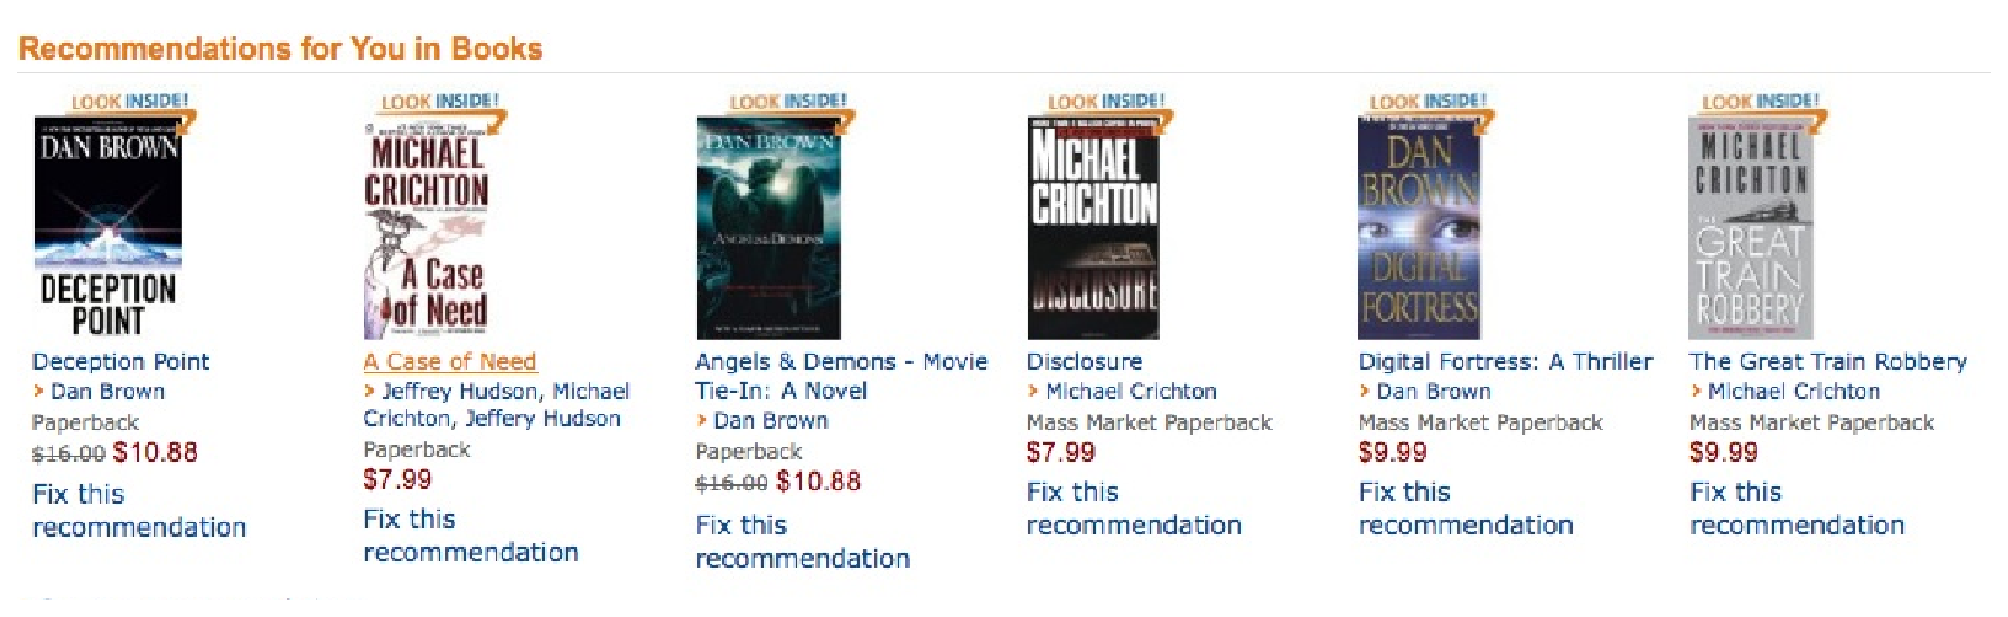
\includegraphics[scale=0.25]{../talk/figures/amazonRecommendations.eps}
\end{figure}
\pitem Can be thought of as link prediction in the affiliation network.
\pitem Can we exploit auxiliary networks (like the friendship network)?
\end{itemize}
\end{frame}

\begin{frame}
\frametitle{Part 2/5}
  \hspace{1.1in}
  \centerline{\huge{Modeling user-affiliation affinity}}
\end{frame}

\begin{frame}
\frametitle{The combined network $\mathcal{C}$}
\tikzstyle{user}=[circle, fill=magenta!25,minimum size=15pt,inner sep=0pt]
\tikzstyle{community}=[circle, fill=cyan!25,minimum size=15pt,inner sep=0pt]
\tikzstyle{userUserEdge} = [draw,thick,-, color=red]
\tikzstyle{userGroupEdge} = [draw,thick,-, color=blue]
\pause
\begin{tikzpicture}[scale=0.8]	
    % Combined network
    \foreach \pos/\name/\user in {{(5,0)/5/Eve}, {(5,1)/4/Dave}, {(5,2)/3/Carol}, {(5,3)/2/Bob},{(5,4)/1/Alice}}
        \node[user] (u\name) [label=left:\user] at \pos {$\name$};
    \foreach \pos/\name/\group in {{(7,0)/6/Tennis}, {(7,1)/5/Math}, {(7,2)/4/Football},{(7,3)/3/Science}, {(7,4)/2/Jazz},{(7,5)/1/Salsa},{(7,-1)/7/Cryptography}}
        \node[community] (c\name)  [label=right:\group] at \pos {$\name$};
    \foreach \source/ \dest in {u1/u2, u1/u3, u1/u4, u2/u4,u1/u5}
       \path (\source) edge [color=red, bend right] (\dest);
    \foreach \source/ \dest in {u1/c1,u1/c4,u2/c1,u3/c5,u3/c6,u4/c2,u1/c7,u2/c7,u3/c7,u4/c7,u5/c3}
        \path[userGroupEdge] (\source) -- (\dest);
    \draw (5,5) node[above]{\large{$\mathcal{C}$}};
   \pause
    % Write the combined adjacency matrix
    \draw (0,2) node[above] {\large{$\bC(\gl, \bD) = \begin{bmatrix} \gl \red{S}& \blue{A}\\ \blue{A^{T}}& \bD\end{bmatrix}$}};
\end{tikzpicture}
\begin{itemize}
 \pitem $\red{S}$: User-User adjacency.
 \pitem $\blue{A}$: User-Affiliation adjacency.
 \pitem $\gl$: relative weight associated with information in $S$.
 \pitem $\bD$: unobserved (choices: $A^{T}A$, \dots).
\end{itemize}
\end{frame}

\begin{frame}
\frametitle{Sub-part 1/2}
  \hspace{1.1in}
  \centerline{\huge{Latent factors model}}
\end{frame}

\begin{frame}
\frametitle{Modeling $\mathcal{A}$ alone}
\begin{itemize}
\pitem User-group affinity as product of low dimensional vectors: $\blue{A}_{i, j} \approx \dprod{\bU(i, :), \bG(i, :)}$.
\pause
\[ \blue{A} \approx \bU \bG^{T} \] 
\[ \text{rank}(\bU) \leq k, \text{rank}(\bG) \leq k \]
$\bU$ - User preferences; $\bG$ - Affiliation characteristics.
\pitem For user $u$, recommend affiliations with high affinity.
\end{itemize}
\end{frame}

\begin{frame}
\frametitle{Modeling $\mathcal{C}$}
\begin{itemize}
\pitem A \textbf{good model} will account for edges in $\red{S}$ too. 
\pause
\[\bC(\gl, \bD) = \begin{bmatrix} \gl \red{S}& \blue{A} \\ \blue{A^{T}}& \bD\end{bmatrix} \approx \begin{bmatrix} \bV_1 \\ \bV_2 \end{bmatrix} \Lambda \begin{bmatrix} \bV_1^{T} & \bV_2^{T} \end{bmatrix}\]
\[\text{rank}(\bV_i) \leq k, \text{rank}(\Lambda) \leq k \]
\pitem So $\blue{A} \approx \bV_1 \Lambda \bV_2^T$.
\pitem $\bV_1 \Lambda \bV_2^T$ is a similarity score matrix for ranking potential affiliations.
\end{itemize}
\end{frame}

\begin{frame}{}
 \frametitle{Sub-part 2/2}
  \hspace{1.1in}
  \centerline{\huge{Graph proximity model}}
\end{frame}

\begin{frame}
\frametitle{Proximity between users in a social network}
\tikzstyle{vertex}=[circle, fill=magenta!25,minimum size=15pt,inner sep=0pt]
\tikzstyle{selected vertex}=[vertex, fill=red]
\tikzstyle{unselect vertex}=[vertex, fill=magenta!25]
\tikzstyle{edge} = [draw,thick,-]
\tikzstyle{selected edge} = [edge,line width=3pt,red!25]
\tikzstyle{unselect edge} = [selected edge, red]

\begin{center}
\begin{tikzpicture}[scale=2]
    % Social network
    \node[vertex] (u4) at (0,1) {};
    \node[vertex] (u3) at (0,2) {$i$};
    \node[vertex] (u2) at (1,1) {$j$};
    \node[vertex] (u1) at (1,2) {};
    \node[vertex] (u5) at (1,3) {};
    
    \foreach \source/ \dest in {u1/u2, u1/u3, u1/u4, u2/u4, u1/u5}
        \path[edge] (\source) -- (\dest);
    \begin{pgfonlayer}{background}
        \pause
        \foreach \source / \dest in {3/1, 1/2}
            \path<+->[selected edge] (u\source) -- (u\dest);
        \foreach \source / \dest / \fr in {3/1/4,1/2/4}
            \path<\fr->[unselect edge] (u\source) -- (u\dest);
    \end{pgfonlayer}
\end{tikzpicture}
\end{center}
\pause
$(\bC^{2})_{i,j}$ : Number of paths of length 2 between $i$ and $j$.
\end{frame}

\begin{frame}
\frametitle{Proximity between users in a social network}
\tikzstyle{vertex}=[circle, fill=magenta!25,minimum size=15pt,inner sep=0pt]
\tikzstyle{selected vertex}=[vertex, fill=red]
\tikzstyle{unselect vertex}=[vertex, fill=magenta!25]
\tikzstyle{edge} = [draw,thick,-]
\tikzstyle{selected edge} = [edge,line width=3pt,red!25]
\tikzstyle{unselect edge} = [selected edge, red]

\begin{center}
\begin{tikzpicture}[scale=2]
    % Social network
    \node[vertex] (u4) at (0,1) {};
    \node[vertex] (u3) at (0,2) {$i$};
    \node[vertex] (u2) at (1,1) {$j$};
    \node[vertex] (u1) at (1,2) {};
    \node[vertex] (u5) at (1,3) {};
    \foreach \source/ \dest in {u1/u2, u1/u3, u1/u4, u2/u4, u1/u5}
        \path[edge] (\source) -- (\dest);

    \begin{pgfonlayer}{background}
        \pause
        \foreach \source / \dest in {3/1,1/4, 4/2}
            \path<+->[selected edge] (u\source) -- (u\dest);
        \foreach \source / \dest / \fr in {3/1/5,1/4/5,4/2/5}
            \path<\fr->[unselect edge] (u\source) -- (u\dest);
    \end{pgfonlayer}
\end{tikzpicture}
\end{center}
\pause
$(\bC^{3})_{i,j}$ : Number of paths of length 3 between $i$ and $j$.
\end{frame}

\begin{frame}
\frametitle{Graph Proximity Model}
\begin{itemize}
\pitem $\text{Proximity}(i, j) = \gb^{2} (\bC^{2})_{i,j} + \gb^{3}(\bC^3)_{i,j} + \dots$
\pitem Known as Katz measure, when the series is convergent, i.e. $\|\gb \bC \|_{2} < 1$.
\pitem A practical and good approximation: Truncated Katz,
\[ \textsf{tKatz}(\bC, \gb, k) = \sum_{i=1}^{k} \gb^i \bC^i. \]
\pitem Recommend affiliations based on proximity in $\bC$.
\end{itemize}
\end{frame}

\begin{frame}
\frametitle{Types of paths considered}
\tikzstyle{user}=[circle, fill=magenta!25,minimum size=15pt,inner sep=0pt]
\tikzstyle{community}=[circle, fill=cyan!25,minimum size=15pt,inner sep=0pt]
\tikzstyle{userUserEdge} = [draw,thick,-, color=red]
\tikzstyle{userGroupEdge} = [draw,thick,-, color=blue]
\pause
\begin{tikzpicture}[scale=0.8]	
    % Combined network
    \foreach \pos/\name/\user in {{(5,0)/5/Eve}, {(5,1)/4/Dave}, {(5,2)/3/Carol}, {(5,3)/2/Bob},{(5,4)/1/Alice}}
        \node[user] (u\name) [label=left:\user] at \pos {$\name$};
    \foreach \pos/\name/\group in {{(7,0)/6/Tennis}, {(7,1)/5/Math}, {(7,2)/4/Football},{(7,3)/3/Science}, {(7,4)/2/Jazz},{(7,5)/1/Salsa},{(7,-1)/7/Cryptography}}
        \node[community] (c\name)  [label=right:\group] at \pos {$\name$};
    \foreach \source/ \dest in {u1/u2, u1/u3, u1/u4, u2/u4,u1/u5}
       \path (\source) edge [color=red, bend right] (\dest);
    \foreach \source/ \dest in {u1/c1,u1/c4,u2/c1,u3/c5,u3/c6,u4/c2,u1/c7,u2/c7,u3/c7,u4/c7,u5/c3}
        \path[userGroupEdge] (\source) -- (\dest);
        \pause
         \draw (5,-3) node[above]{$\text{Eve } \, \red{\xrightarrow{S}}\, \text{Alice } \,\blue{\xrightarrow{A}} \, \text{ Cryptography}$ (in $\bC^2$)};
         \pause
         \draw (5,-4) node[above]{$\text{Eve } \, \red{\xrightarrow{S}} \, \text{Alice } \, \xrightarrow{AA^T} \, \text{Bob }\, \blue{\xrightarrow{A}}\, \text{ Cryptography}$ (in $\bC^4$)};
\end{tikzpicture}
\end{frame}


\begin{frame}
\frametitle{Part 3/5}
  \hspace{1.1in}
  \centerline{\huge{Scalability}}
\end{frame}

\begin{frame}
\frametitle{Real world networks are huge!}
\begin{itemize}
\pitem \emph{Orkut} (sub)network [Mislove,2007] is about 3 million users and 8 million groups.
\pitem Recall $\textsf{tKatz}(\bC, \gb, k) = \sum_{i=1}^{k} \gb^i \bC^i $.
\pitem $\bC^i$ gets denser --- prohibitively expensive computations and memory usage. 
\end{itemize}
\end{frame}

\begin{frame}
\frametitle{So how does the model scale?}
\begin{itemize}
\pitem A plausible solution...
\pitem Use low rank approximations --- $\bC \approx \bV\Lambda \bV^{T}$. 
\pitem Then, $\bC^i \approx \bV\Lambda^{i}\bV^{T}$. [Submitted] % \cite{vasukiScalableAffiliationRec}
\end{itemize}
\end{frame}

\begin{frame}
\frametitle{Smarter solutions...}
\begin{itemize}
\pitem $\textsf{tKatz}(\bC;\gb,3)_{12} = \gb \blue{A} + \gb^2 \lambda \red{S} \blue{A} +  \gb^3(\lambda^2 \red{S}^2 \blue{A} + \blue{A} \blue{A^T} \blue{A})$.
\pitem $(\blue{A}\blue{A^{T}})^i, \red{S}^{i}, (\blue{A}\blue{A^{T}})^{j}\red{S}^{i}$ get denser.
\pause
\begin{align*}
\blue{A} = U_{A} \Sigma_{A} V_{A}^{T}\\
\red{S} = U_{S} \Sigma_{S} U_{S}^{T}
\end{align*}
\pitem Approximate $\blue{A}$ and $\red{S}$ using common subspace of $U_{A}$ and $U_{S}$.
\pause
\begin{align*}
\blue{A} \approx \green{Q} \blue{D_{A}}V^{T} \\
\red{S} \approx \green{Q} \red{D_{S}} \green{Q^{T}}\\
\green{Q} = f(U_{A}, U_{S}), \green{Q^{T}}\green{Q} = I, V^{T}V = I
\end{align*}
\pitem Efficiently compute the terms now! e.g. $(\blue{A}\blue{A^{T}})^j\red{S}^{i} \approx \green{Q}(\blue{D_A}\blue{D_A^{T}})^{j}\red{D_{S}}^{i} \green{Q^T}$.
\pitem Clustered low-rank approximations [Submitted].
\end{itemize}
\end{frame}

\begin{frame}
\frametitle{Part 4/5}
  \hspace{1.1in}
  \centerline{\huge{Evaluation of the algorithms}}
\end{frame}

\begin{frame}
\frametitle{Data sets}
Extracted social and affiliation networks: \emph{Orkut} and \emph{Youtube} data sets [Mislove,2007]; Orkut: \blue{$N_{u} = 9123, N_{g} = 75546$}. Youtube: \blue{$N_{u} =16575, N_{g} = 21326$}.
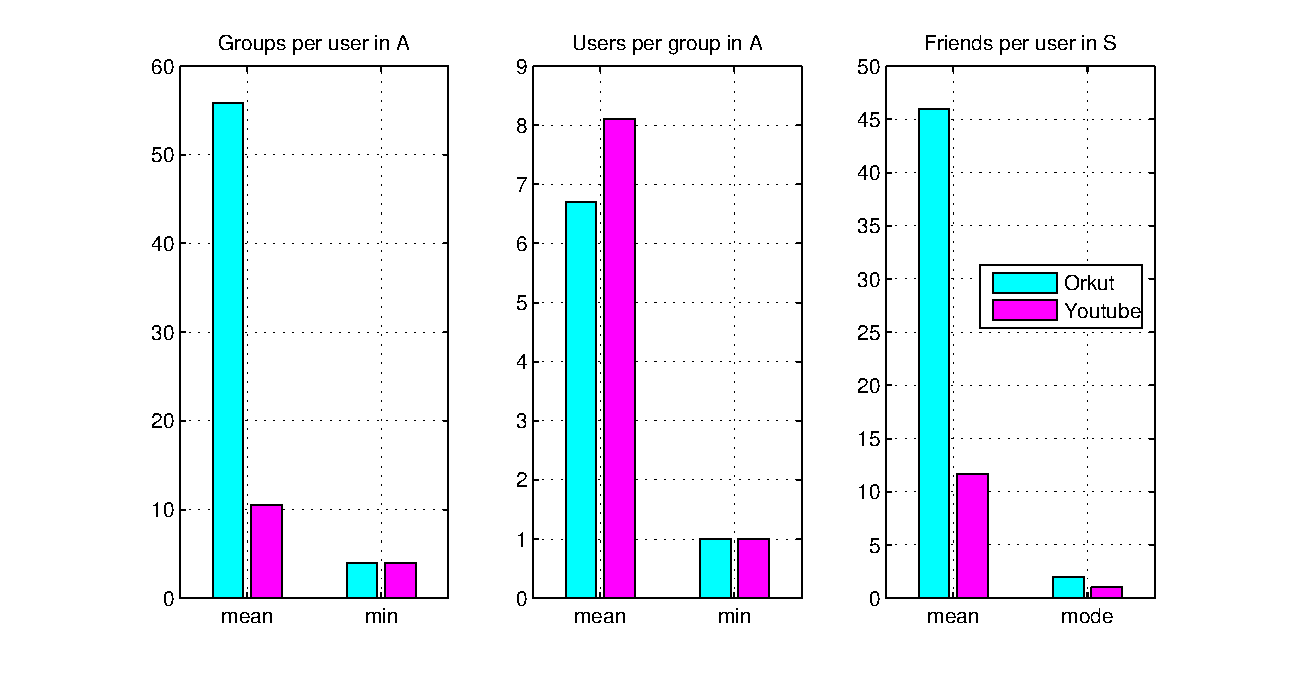
\includegraphics[scale=0.5]{../talk/figures/stats.eps}
\end{frame}

\begin{frame}
\frametitle{Evaluation methods}
\begin{itemize}
\pitem Choosing appropriate evaluation method --- Depends on the end user of the recommendation system.
\pitem ``Global'' sensitivity vs ``Per-user'' sensitivity.
\pitem Using Global sensitivity...
\pause
\begin{figure}[h]
  \begin{center}
    \subfigure[Orkut dataset]{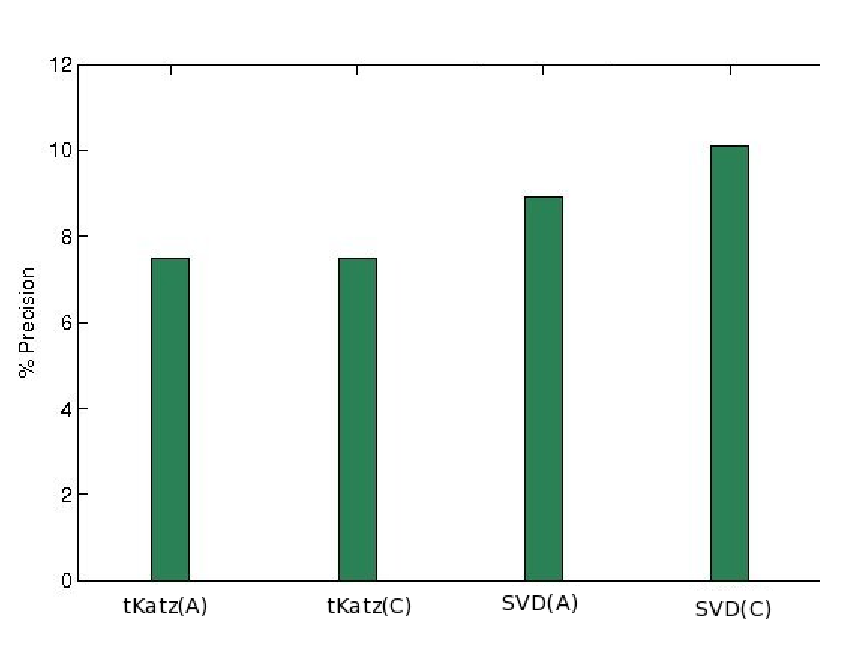
\includegraphics[scale=0.25]{../paper/OrkutLinkPredictionEvaluation.eps}}
    \subfigure[Youtube dataset]{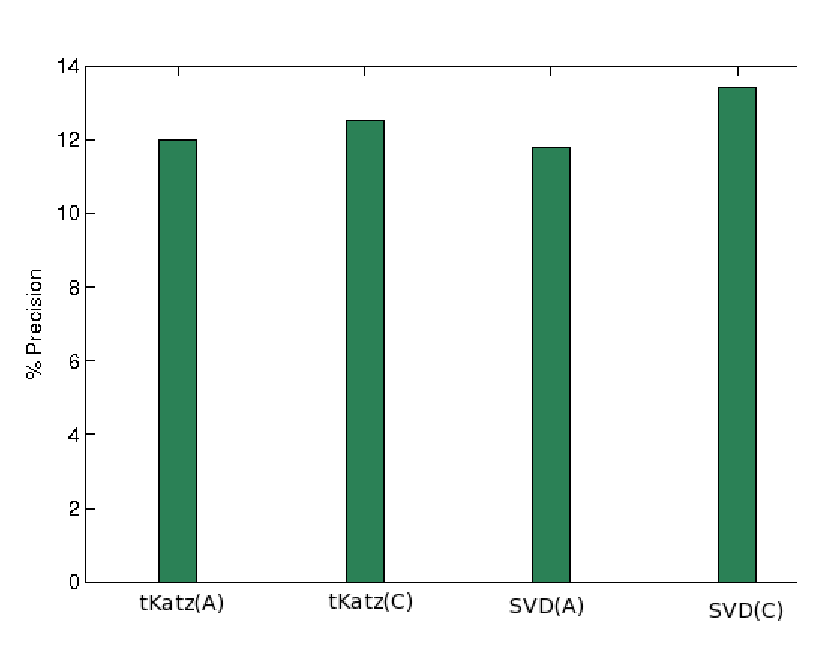
\includegraphics[scale=0.25]{../paper/YoutubeLinkPredictionEvaluation.eps}}
  \end{center}
\end{figure}
\end{itemize}
\end{frame}

\begin{frame}
\frametitle{Results: ``Per-user'' sensitivity}
Consider the top $k$ recommendations made for a user for $k = 5, 10, \dots, 50$.
\begin{figure}[h]
  \begin{center}
    \subfigure[Orkut dataset]{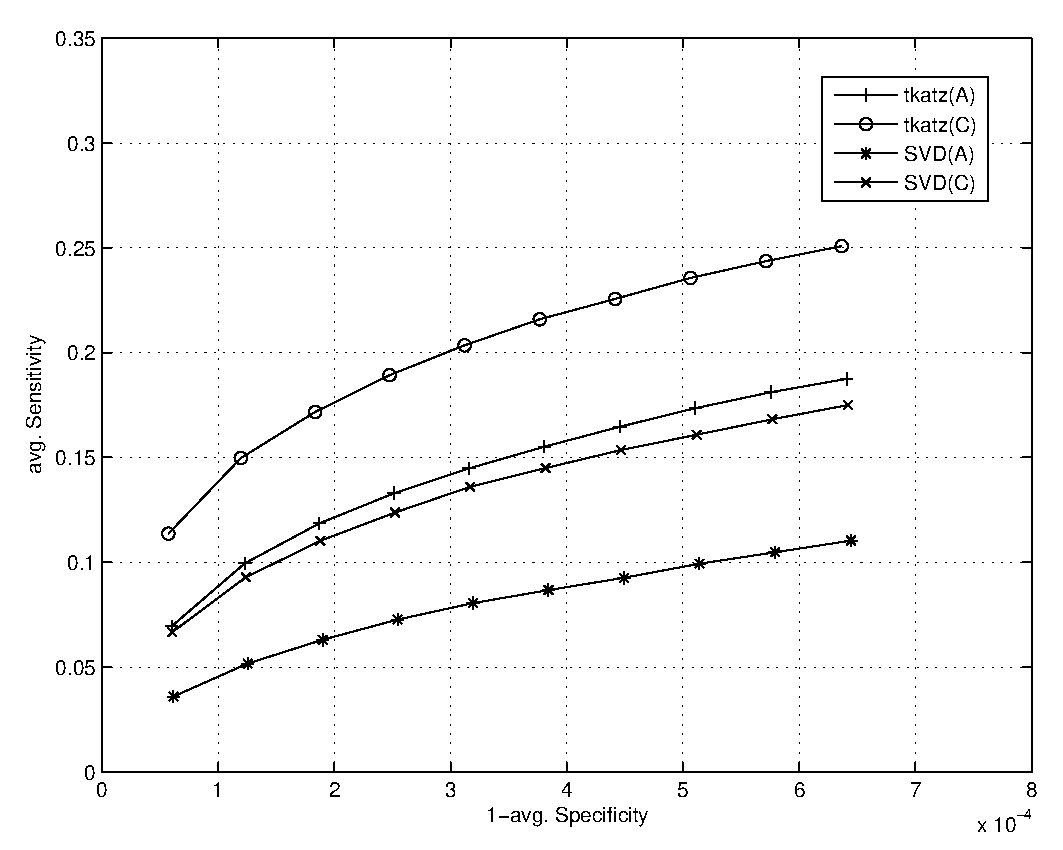
\includegraphics[scale=0.3]{../paper/summaryOrkut.eps}}
    \subfigure[Youtube dataset]{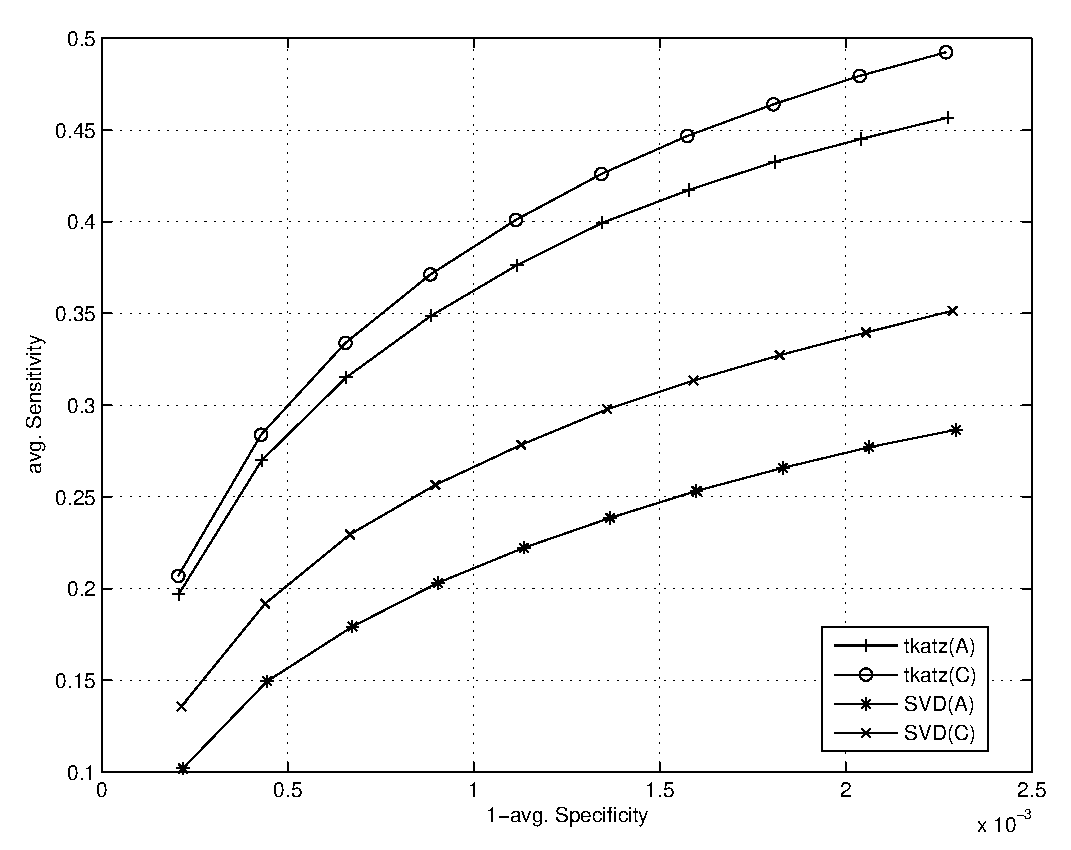
\includegraphics[scale=0.3]{../paper/summaryYoutube.eps}}
  \end{center}
\end{figure}
\end{frame}

\begin{frame}
\frametitle{Similarity between affiliations in the combined network?}
\pause
\center{Recall $\bC = \begin{bmatrix} \gl \red{S}& \blue{A} \\ \blue{A^{T}}& \bD\end{bmatrix}$}
\center{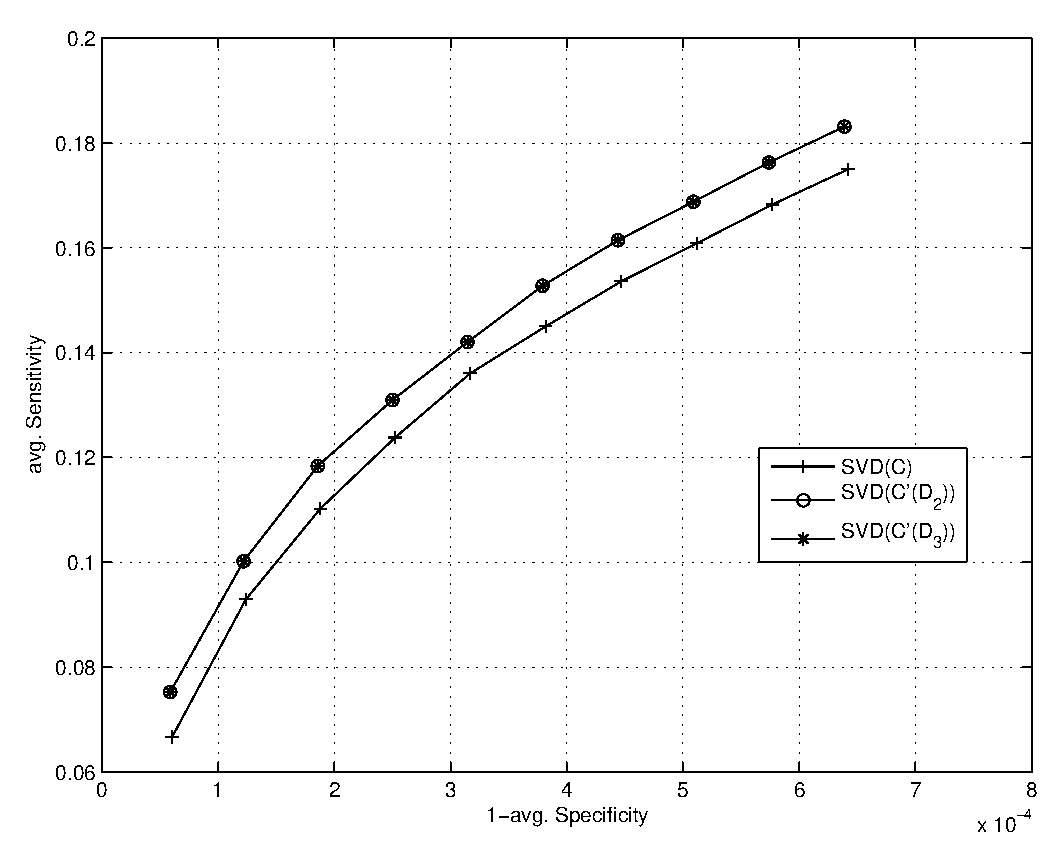
\includegraphics[scale=0.4]{../paper/summarySVDOrkut.eps}}
\pause
$\bD = 0, \bD_{2} = \bA^{T}\bA, \bD_{3} = \lambda \bA^{T}\bA$. \\
\pause
Information from $\bD$ may be redundant!
\end{frame}

\begin{frame}
\frametitle{Scalable approximations: Youtube}
\begin{center}
\includegraphics[scale=0.4]{../journalPaper/summarySVDKatzYoutube.eps}
\end{center}
\pause
\textsf{tKatzLFM}: \textsf{tKatz} on low-rank approximation.\\
\pause
\textsf{tKatzCS}: \textsf{tKatz} on low-rank approximation using common subspace.\\
\pause
and other clustered approximation variants...
\end{frame}

%\begin{frame}
%\frametitle{Results}
%\begin{figure}
%  \begin{center}
%    \subfigure[Orkut-1c data set]{\includegraphics[scale=0.25]{../journalPaper/summaryScalabilityOrkut.eps}}
%    \subfigure[Youtube-1c data set]{\includegraphics[scale=0.25]{../journalPaper/summaryScalabilityYoutube.eps}}
%  \end{center}
%  \caption{Scalable approximations: Clustering}
%\end{figure}
%\end{frame}

\begin{frame}
\frametitle{Quality of approximations}
\begin{center}
\includegraphics[scale=0.4]{../journalPaper/summaryRankDependencyYoutube.eps}
\end{center}
\end{frame}

\begin{frame}
\frametitle{Part 5/5}
  \hspace{1.1in}
  \centerline{\huge{Conclusions}}
\end{frame}

\begin{frame}
\frametitle{Summary}
\begin{itemize}
\pitem Friendship network is indeed useful in recommending affiliations!
\pitem Community recommendation -- link prediction perspective.
\pitem Two ways of modeling the information from auxiliary networks --- Latent Factor and Graph Proximity models.
\end{itemize}
\end{frame}

\begin{frame}
\frametitle{Future work}
\begin{itemize}
\pitem Using affiliation networks for link prediction in friendship networks -- Seems harder.
\pitem More sources of information -- How do you use them all?
\pitem More scalable models.
\end{itemize}
\end{frame}

%\begin{frame}
%\frametitle{The take home message}
%\centerline{\huge{Friendship networks can be fruitfully exploited in recommending affiliations.}}
%\end{frame}
\begin{frame}
\frametitle{References}
\begin{itemize}
\item Vishvas Vasuki, Nagarajan Natarajan, Zhengdong Lu, Inderjit Dhillon. \blue{Affiliation recommendations using auxiliary networks}. RECSYS, 2010.
\item Vishvas Vasuki, Nagarajan Natarajan, Zhengdong Lu, Berkant Savas, Inderjit Dhillon. \blue{Scalable affiliation recommendations using auxiliary networks}. Submitted to Transactions on Intelligent Systems and Technology, 2010.
\item Alan Mislove etal. \blue{Measurement and analysis of online social networks}, \emph{In IMC '07: Proceedings of the 7th ACM SIGCOMM Conference on Internet Measurement}, pages 29-42, NY, USA, 2007. ACM.
\end{itemize}
\end{frame}

\begin{frame}{}
  \hspace{1.1in}
  \centerline{\huge{Thank you!}}
\end{frame}

%\bibliographystyle{plain}
%\bibliography{../paper/references}

%
\end{document}
